%% Compile with       pdflatex --jobname=demo-prot1-fig demo-prot1.tex

\documentclass{article}

\usepackage{amsmath}
\usepackage{amstext}
\usepackage{amssymb}
\usepackage{amsfonts}
\usepackage{xspace}
\usepackage{graphicx}
\usepackage{url}
\usepackage{mdwlist}
\usepackage{courier}
\usepackage{lscape}
\usepackage{comment}
\usepackage{wrapfig}
\usepackage{multirow}
\usepackage{bussproofs}
\usepackage{pdftricks}
\usepackage{cite}
\usepackage{footmisc}
\usepackage{balance}
\usepackage{enumerate}
\usepackage[normalem]{ulem}
\usepackage{hyperref}
\usepackage{tikz}
\usetikzlibrary{calc,backgrounds,automata,arrows}
\pgfrealjobname{demo-prot2-s-1}

\begin{document}

\beginpgfgraphicnamed{demo-prot2-s-1-fig}
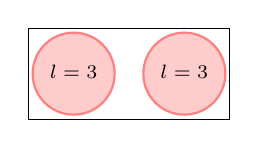
\begin{tikzpicture}
 \tikzstyle{arrow} = [->,shorten >=1pt,>=stealth'];
 \tikzstyle{circles} = [circle,thick,node distance=4em,inner sep=0.05em];
 \tikzstyle{state}   = [matrix,node distance=6em,inner sep=0.1em];
 \tikzstyle{placez} = [node distance=5em,inner sep=0.2em];
 \tikzstyle{placeZ1} = [draw=black,fill=white];
 \tikzstyle{placeZ2} = [draw=black,fill=white];
 \tikzstyle{placeY} = [draw=black,fill=white];
 \tikzstyle{placeB} = [draw=blue!50,fill=blue!20];
 \tikzstyle{placeR} = [draw=red!50,fill=red!20];
 \tikzstyle{placeG} = [draw=green!50,fill=green!20];
 \tikzstyle{placeW} = [draw=black!50,fill=black!10];

 %\node[matrix,name = zbox] {
 %  \node[placez,placeZ1,name=z1] {z1};  
 %  \node[placez,placeZ2,name=z2, right of=z1] {z2}; \\
 %};

 %% node [0]
 \node[state, name = node0] {
   \node[circles,placeR,name=s00] {\scriptsize 
                                                $
                                                 \begin{array}{l}
			                           l = 3
			                         \end{array}
			                        $};
   \node[circles,placeR,name=s01, right of=s00] {\scriptsize
                                                 $
                                                 \begin{array}{l}
			                           l = 3
			                         \end{array}
			                        $}; \\
 };
 \draw (node0.north west) rectangle (node0.south east);

 %\path (node0) edge [arrow, bend left] node [below] {} (node0);

\end{tikzpicture}
\endpgfgraphicnamed

\end{document}


